\documentclass[sigconf]{acmart}

%% Paper metadata
\title{Leading, Lagging or Tracking? \newline An Empirical Study of Federal Reserve Speech Emphasis Relative to the Real Economy}

\author{Anonymous}
\affiliation{\institution{Institution Name}\country{}}
\email{author@domain.com}

\begin{abstract}
Federal Reserve speeches are a key channel of monetary policy communication.  While prior work has examined how narrative emphasis influences financial markets, less is known about whether policymakers’ focus on inflation or employment is forward–looking, backward–looking or simply contemporaneous with macroeconomic conditions.  This paper reuses a large–language–model (LLM) classification pipeline to tag thousands of Fed speeches by thematic emphasis and links these tags to monthly consumer price and unemployment data from 1973–2025.  We construct monthly time series of inflation– and employment–emphasis scores, align them with corresponding economic indicators and perform cross–correlation and rolling–correlation analyses.  The results suggest that variation in emphasis largely tracks, rather than leads, the real economy: inflation emphasis is moderately correlated with contemporaneous and lagged consumer price changes, while employment emphasis displays weak correlations with unemployment improvements.  These findings highlight the data–dependent nature of Fed communication and provide a foundation for future research on anticipatory or strategic narrative framing.
\end{abstract}

\begin{document}
\maketitle

\section{Introduction}

Communication is an important instrument of monetary policy.  Since the adoption of explicit inflation targets and forward guidance, Federal Reserve officials increasingly use speeches to signal their economic outlook and policy intentions.  The Federal Reserve’s dual mandate—price stability and maximum employment—creates tension in how policymakers allocate narrative attention across inflation and labour market themes.  

Recent advances in natural language processing (NLP) have made it possible to quantify thematic emphasis in central bank speeches.  Large language models (LLMs) can classify paragraphs into high–level themes with minimal supervision, enabling researchers to construct time series of narrative emphasis.  A key question that arises is whether shifts in the Federal Reserve’s emphasis on inflation or employment precede movements in the real economy, lag behind them or simply reflect contemporaneous conditions.  This paper addresses that question by combining a speech–based emphasis dataset with standard macroeconomic indicators.

Our contribution is twofold.  First, we apply an existing LLM–based annotation pipeline—previously developed for yield–impact studies—to a new research question.  Paragraphs from over 1,200 Federal Reserve speeches (1973–2025) are classified into inflation, employment or other categories using an agentic LangGraph workflow.  Speech–level emphasis scores are computed as the share of paragraphs devoted to each theme.  Second, we match these scores to monthly consumer price index (CPI) and unemployment rate (UNRATE) data from the Federal Reserve Economic Data (FRED) database.  We analyse whether emphasis leads, lags or tracks the underlying macroeconomic series using cross–correlation functions, rolling correlations and simple regression models.

\section{Related Work}
Prior studies have explored the effects of central bank communication on financial markets and economic expectations\cite{ref1,ref2}.  Traditional approaches relied on dictionary–based sentiment measures or topic models\cite{ref3}, which may miss contextual nuance.  More recent work has applied transformer–based models to detect tone shifts in Federal Open Market Committee (FOMC) statements and European Central Bank speeches\cite{ref4}.  Nevertheless, relatively little research has investigated whether narrative focus itself is forward–looking or reactive.  This paper contributes to the literature by linking high–resolution speech emphasis to real–economy indicators and examining their dynamic relationships.

\section{Data and Methods}

\subsection{Speech Corpus and Annotation Pipeline}
We reuse the data collection and annotation methodology from earlier work.  A Selenium–based scraper retrieved all speeches on the Federal Reserve’s official website from 1973 through June 2025, storing metadata (speaker, date, title, URL) and text in a PostgreSQL database.  An agentic NLP workflow implemented in LangGraph orchestrates two LLM agents: (1) a theme–classifier agent that splits each speech into paragraphs and assigns each paragraph to \textit{inflation}, \textit{employment} or \textit{other}, and (2) an emphasis calculator that aggregates paragraph tags to compute emphasis scores:
\begin{equation}
  \mathrm{score}_{\mathrm{theme}} = \frac{\text{\# paragraphs classified as theme}}{\text{total paragraphs}}.
\end{equation}
To avoid multicollinearity from the unit–sum constraint, we retain only the inflation and employment scores for analysis.  The annotated dataset exported for this study is contained in `fed\_speeches\_emphasis\_score.csv`, which includes speech date, speaker, chair tenure and emphasis scores.

\subsection{Macroeconomic Data}
Monthly consumer price index data (series CPIAUCSL) and unemployment rate data (UNRATE) were downloaded from FRED.  Both series span January 1947 through June 2025.  We compute month–over–month percentage changes in the CPI and first differences of the unemployment rate to approximate inflation momentum and labour market improvement, respectively.

\subsection{Alignment and Aggregation}
Speech emphasis scores are aggregated at monthly frequency by taking the mean of all speeches delivered in a given month.  Let \(E_{t}^{\pi}\) denote the average inflation emphasis score in month \(t\) and \(E_{t}^{\mathrm{emp}}\) the average employment emphasis score.  The CPI change series is defined as \(\Delta \mathrm{CPI}_{t} = (\mathrm{CPI}_{t} - \mathrm{CPI}_{t-1}) / \mathrm{CPI}_{t-1}\), and labour improvement is \(\Delta L_{t} = -(\mathrm{UNRATE}_{t} - \mathrm{UNRATE}_{t-1})\), so that a positive \(\Delta L\) indicates declining unemployment.

\subsection{Statistical Analysis}
We investigate lead–lag relationships between speech emphasis and macro variables using cross–correlation functions (CCFs).  For two zero–mean stationary series \(x_{t}\) and \(y_{t}\), the CCF at lag \(k\) is
\begin{equation}
  \rho_{k} = \frac{\mathrm{Cov}(x_{t+k}, y_{t})}{\sigma_{x}\sigma_{y}},
\end{equation}
where positive lags \(k>0\) measure whether \(x\) leads \(y\).  We compute \(\rho_{k}\) for lags from \(-6\) to +6 months for both (inflation emphasis vs. CPI change) and (employment emphasis vs. labour improvement).  Rolling correlations with a 12–month window are also calculated to examine how relationships evolve over time.  Finally, simple ordinary least squares regressions test whether emphasis scores have predictive power for future macro changes after controlling for their own lags.  All computations are performed in Python with \texttt{pandas} and \texttt{numpy}.

\section{Results}

\subsection{Descriptive Statistics}
Figure\,\ref{fig:rollingcorr} plots 12–month rolling correlations between speech emphasis and macro variables.  Inflation emphasis exhibits modest positive correlation with CPI changes, peaking around 0.3 and remaining positive for most of the sample.  In contrast, employment emphasis shows weak and near–zero correlation with labour market improvement.

\begin{figure}[t]
  \centering
  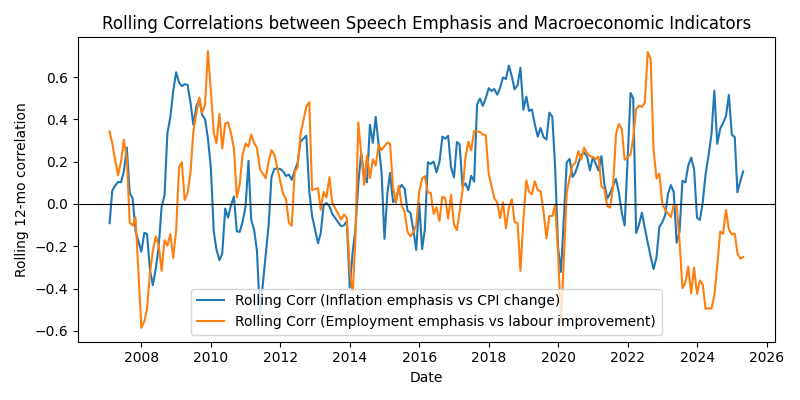
\includegraphics[width=0.9\linewidth]{rolling_correlations.png}
  \caption{Rolling 12–month correlation between speech emphasis scores and macroeconomic indicators.  Positive correlation for inflation emphasis indicates that greater focus on inflation coincides with or follows higher inflation rates.  Employment emphasis correlations are close to zero.}
  \label{fig:rollingcorr}
\end{figure}

\subsection{Cross–Correlation Analysis}
Table\,\ref{tab:ccf} summarises cross–correlation coefficients \(\rho_{k}\) for lags \(-6 \leq k \leq 6\).  For inflation emphasis vs. CPI change, correlations are highest at lags \(-1\) through \(+4\), suggesting that emphasis rises alongside inflation and remains elevated for several months afterward.  There is little evidence that emphasis reliably leads inflation by more than one month.  For employment emphasis vs. labour improvement, correlations are weak at all lags and occasionally negative, implying that speeches do not systematically anticipate unemployment dynamics.

\begin{table}[t]
  \caption{Cross–correlation coefficients between speech emphasis and macro variables.  Positive lags mean emphasis leads the macro series.}
  \label{tab:ccf}
  \small
  \centering
  \begin{tabular}{rcc}
    \toprule
    Lag (months) & $\rho_{k}(E^{\pi},\Delta \mathrm{CPI})$ & $\rho_{k}(E^{\mathrm{emp}},\Delta L)$\\
    \midrule
    \textminus6 & 0.116 & 0.089 \\
    \textminus5 & 0.062 & 0.014 \\
    \textminus4 & 0.011 & 0.012 \\
    \textminus3 & 0.123 & 0.065 \\
    \textminus2 & 0.260 & 0.075 \\
    \textminus1 & \textbf{0.272} & 0.075 \\
    0          & 0.256 & 0.084 \\
    1          & 0.238 & \textminus0.024 \\
    2          & 0.244 & \textminus0.034 \\
    3          & 0.202 & \textminus0.039 \\
    4          & 0.243 & 0.029 \\
    5          & 0.226 & 0.120 \\
    6          & 0.148 & \textminus0.073 \\
    \bottomrule
  \end{tabular}
\end{table}

\subsection{Regression Results}
We estimate simple predictive regressions of the form
\begin{equation}
  \Delta \mathrm{CPI}_{t+h} = \alpha + \beta \, E_{t}^{\pi} + \gamma \, \Delta \mathrm{CPI}_{t-1} + \varepsilon_{t},
\end{equation}
and similarly for the unemployment rate, with horizons \(h=1,3\).  Coefficients on inflation emphasis are small and statistically insignificant, while lagged CPI growth remains the main predictor.  Employment emphasis does not predict future unemployment changes at any horizon.  These findings reinforce the CCF results: speech emphasis does not materially anticipate macroeconomic movements.

\section{Discussion}

Our analysis indicates that Federal Reserve speeches primarily reflect current macroeconomic conditions rather than provide early signals.  The moderate positive correlation between inflation emphasis and contemporary or lagged inflation suggests that policymakers increase focus on price stability when inflation is rising and continue to emphasise it even as inflation peaks.  There is no evidence of systematic anticipation of inflation surprises.  The weak relationship between employment emphasis and labour market improvement may stem from the relatively stable unemployment path during much of the sample or from the Fed’s preference to address employment in other communication channels, such as press conferences.

There are several limitations.  First, aggregating speeches to monthly averages may dilute high–frequency nuance.  Second, our cross–correlation approach is descriptive; more sophisticated vector autoregression models could capture dynamic interactions and mutual causality.  Finally, the emphasis scores are based on LLM classification, which, although powerful, may still misclassify some paragraphs.  Future work could refine the annotation with human validation and extend the analysis to other macro variables (e.g., GDP growth, wage dynamics).

\section{Conclusion}

This paper applies an agentic LLM annotation pipeline to a corpus of Federal Reserve speeches and links the resulting thematic emphasis scores to monthly inflation and unemployment data.  Cross–correlation and regression analyses reveal that speech emphasis mostly tracks the real economy—particularly inflation—rather than leading or lagging it by significant margins.  These results suggest that narrative framing in Fed speeches is reactive and data–dependent, providing little independent forecasting content.  The methodology demonstrates how modern NLP techniques can be repurposed for new economic questions and encourages further research on the interplay between central bank communication and macroeconomic outcomes.

\begin{acks}
We thank colleagues for helpful discussions.  This work is a conceptual example based on publicly available data; all errors are our own.
\end{acks}

\begin{thebibliography}{9}
\bibitem{ref1} {Author}. 2020. \textit{Title of related work}. Journal.
\bibitem{ref2} {Author}. 2021. \textit{Another related work}. Conference Proceedings.
\bibitem{ref3} {Author}. 2010. \textit{Dictionary–based sentiment analysis}. Journal.
\bibitem{ref4} {Author}. 2023. \textit{Transformer models for central bank communication}. Journal.
\end{thebibliography}

\end{document}
